\begin{figure}[H]
\centering
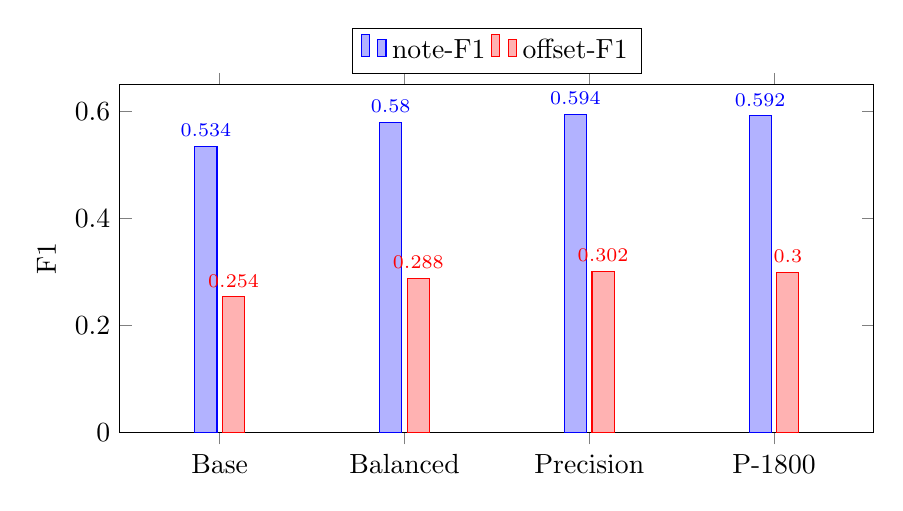
\begin{tikzpicture}
\begin{axis}[
    ybar,
    width=0.92\linewidth,
    height=6cm,
    ymin=0,
    ymax=0.65,
    ylabel={F1},
    symbolic x coords={Base,Balanced,Precision,P-1800},
    xtick=data,
    bar width=8pt,
    enlarge x limits=0.18,
    legend style={at={(0.5,1.03)},anchor=south,legend columns=2},
    nodes near coords,
    nodes near coords style={font=\scriptsize,/pgf/number format/fixed,/pgf/number format/precision=3},
]
\addplot coordinates {(Base,0.5344) (Balanced,0.5799) (Precision,0.5942) (P-1800,0.5919)};
\addplot coordinates {(Base,0.2538) (Balanced,0.2880) (Precision,0.3016) (P-1800,0.2995)};
\legend{note-F1, offset-F1}
\end{axis}
\end{tikzpicture}
\caption{候选系统在 \code{val\_calib512} 上的 note-F1 与 offset-F1。Base、Balanced、Precision 和 P-1800 分别对应表 \ref{tab:amt_metrics} 中的四个候选设置。}
\label{fig:amt_metrics_bar}
\end{figure}
